
\graphicspath{ {./Pictures/} }
%----------------------------------------------------------------------------------------
%	CHAPTER 3
%----------------------------------------------------------------------------------------

\chapterimage{boat.png}
\chapter{Calculus}



\section{Differentiation}
	In mathematics, differential calculus is a subfield of calculus concerned with the study of the rates at which quantities change.
	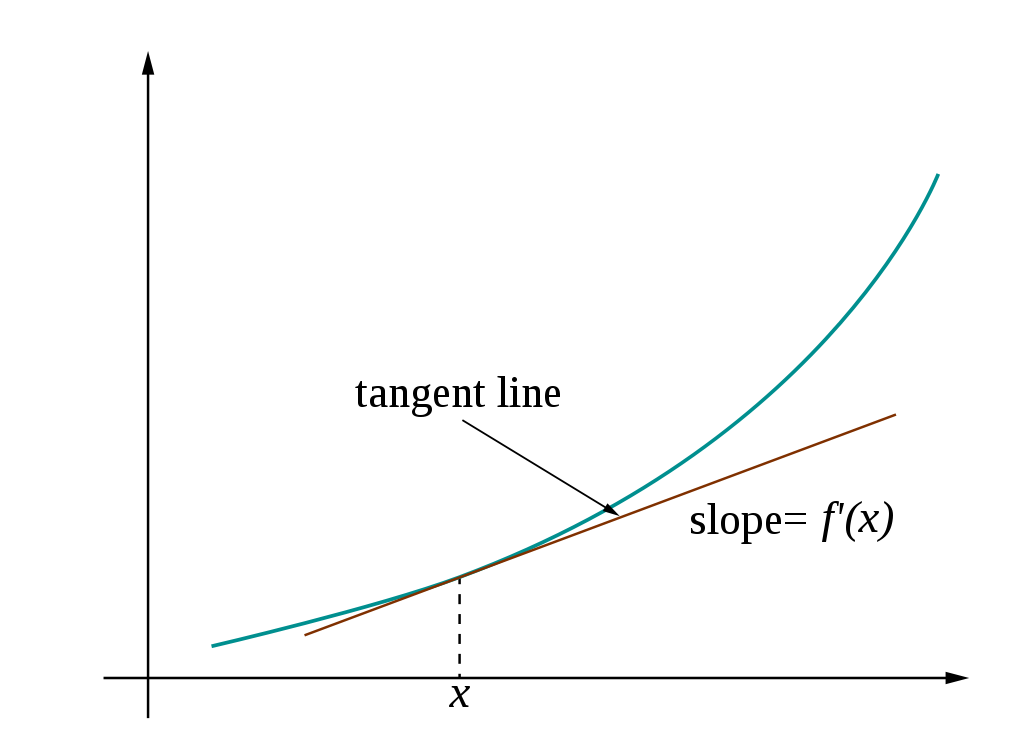
\includegraphics[width=50mm]{02}
	It is one of the two traditional divisions of calculus, the other being integral calculus, the study of the area beneath a curve.
	
	
	\begin{equation}
		\frac{duv}{dx}=\frac{du}{dx}v+u\frac{du}{dx}
	\end{equation}
	\begin{align}
		\frac{df(x)}{dx} = \frac{f(x+h)-f(x)}{h} \\
		\frac{(f+df)-(f)}{dx}	\\
		\frac{df}{dx} \\
	\end{align}
	
	\begin{align}
		\frac{duv}{dx} = \frac{(u+du)(v+du)-uv}{dx} \\
		=>\frac{(uv+du+udv+dudv)-uv}{dx} \\
		=> \frac{duv+duv+dudv}{dx} \\
		=> \frac{duv+udv}{dx} \\
		=> \frac{du}{dx}v+u\frac{dv}{dx} \\
	\end{align}
	\begin{align}
		\frac{df}{dx} = \frac{f_2-f_1}{x_2-x_1} \\\\
		=>\frac{(f_1+df)-f_1}{x_2-x_1} \\
		=>\frac{(f_1+df)-f_1}{dx} \\
	\end{align}

	
	
	
	\subsection{Differentiation of trigonometric functions}
	\begin{equation}
		\sin(A+B) = \sin A\cos B+\cos A\sin B
	\end{equation}
	\begin{equation}
		\cos(A+B) = \cos A\cos B - \sin A\sin B
	\end{equation}
	\begin{equation}
		\frac{df(x)}{dx} = \frac{f(x+h)-x}{h}
	\end{equation}
		
	Example: 1
	\begin{align}
		\frac{d\sin(x)}{dx} = \frac{\sin x \cos h+\cos x\sin h-\sin x}{h} \\
		=> \frac{\sin x + h\cos x - \sin x}{h} \\
		=>\frac{h\cos x}{h} \\
		\frac{d\sin(x)}{dx} = \cos x \\
	\end{align}
	
	Example: 2
	\begin{align}
		\frac{d\cos(x)}{dx} = \frac{\cos(c+h)-\cos (x)}{h} \\
		=> \frac{\cos x \cos h-\sin x \sin h - \cos x}{h} \\
		=> \frac{cos x- h \cos x - \cos x}{h} \\
		=> \frac{-h\sin x}{h} \\
		\frac{d\cos (X)}{dx} = -\sin x \\
	\end{align}
	
	Example: 3
	\begin{align}
		\frac{d\tan x}{dx} \\
		=>\frac{d}{dx}\bigg(\frac{\sin x}{cos x}\bigg) \\
		=>\frac{d}{dx}(\sin x)\frac{1}{\cos x}+\sin x \frac{d}{dx}\bigg(\frac{1}{\cos x}\bigg)\\
		=>\cos x \frac{1}{\cos x}+\sin x\frac{d}{dx}(\cos x)^{-1} \\
		=> 1+\sin x\bigg[(-1)(\cos x)^{-2}\frac{d\cos x}{dx}\bigg] \\
		=> 1+\sin x\frac{-1}{\cos x^2}(-\sin x) \\
		\frac{d \tan x}{dx} = 1 + \tan^2 x \\
	\end{align}


	\subsection{Properties of Differential Operator}
	
	
	
	
	\subsection{Chain Rule}
	
	\begin{align}
		\frac{df(g(x))}{dx} = \frac{df(g(x))}{dg(x)}\frac{dy(x)}{dx}  \\
		\frac{df(g(x))}{dx} = \frac{df(x)}{dy}\frac{dg(x)}{dx} \\
	\end{align}	

	Example: 1
	\begin{align}
		Proof\,that\, \quad\frac{de^{x^2}}{dx} = 2x \, e^{x^2} \\
		Let, \quad x^2 = y \\
		=> \frac{de^2}{dx} \\
		=> \frac{de^y}{dy}\frac{dy}{dx} \\
		e^y\frac{dx^2}{dx} \\
		e^y\,2x \\
		=> 2x\,e^{x^2} \\
	\end{align}

	Example: 2
	\begin{align}
		\frac{d\sin(x^3)}{dx} \\
	 	=> \frac{d \sin(x^3)}{dx}\frac{d(x^3)}{dx} \\
	 	=> \cos(x^3) \,3x^2 \\
	\end{align}	 


	\begin{equation}
		\frac{d(2x^2)}{dx} = \frac{2(x+h)^2-2x^2}{h} = 2\Big[\frac{(x+h)^2-x^2}{h}\Big] = 2\frac{dx^2}{dx}=2.2x=4x
	\end{equation}
	\begin{equation}
		\frac{d(cf(x))}{dx} = c\frac{df(x)}{dx}\quad (c)\,\,is\,\,a\,\,number 
	\end{equation}
	\begin{equation}
		\frac{d}{dx}\bigg(c_1f(x)+c_2f(x)\bigg)=\frac{d}{dx}\bigg((c_1+c_2)f(x)\bigg)
	\end{equation}
	\begin{equation}
		\frac{d}{dx}\bigg(c_1u(x)+c_2v(x)\bigg)=c_1\frac{du(x)}{dx}+c_2\frac{dv(x)}{dx}
	\end{equation}
		c, are number. f(x), u(x), v(x) are function	
	\newline
	\begin{equation}
		\frac{d\sin(2x^3)}{dx} = \frac{d\sin(2x^3)}{d2x^3}\frac{dx^3}{dx} = \cos(2x^3)\frac{2(x+h)^3-22x^3}{h}=\cos(2x^3)2\frac{dx^3}{dx}=\cos(2x^3)2\,3x^3=\cos(2x^3)6x^3
	\end{equation}
	\begin{equation}
		\frac{de^{\sin(3x)}}{dx}=\frac{de^{\sin(3x)}}{d\sin(3x)}\frac{d\sin(3x)}{dx}=e^{\sin(3x)}\frac{d\sin(3x)}{d3x}\frac{d3x}{dx} = e^{\sin(3x)}\cos(3x)3x
	\end{equation}
	
	
	
	
	
	
	\subsection{Differentiation of Fundamental Functions}
	
		\subsubsection{Powers $x^n$}
		\subsubsection{Exponentials $a^x$}
		\subsubsection{Logarithm $\log_{b} x$}
		
			Example: 1
			\begin{align}
				If \quad y = \log e^x \\
				=> e^y=e^{(10ye^x)} = x \\
				=> \frac{de^x}{dx} = \frac{dx}{dx} = 1 \\
				=>\frac{de^y}{dx} \frac{dy}{dx} = 1 \\
				=>e^y \frac{dy}{dx} = 1 \\
				=>e^{-y}e^y\frac{dy}{dx} = e^{-y} \\
				=>e^{-y+y}\frac{dy}{dx} = e^{-y} \\
				=>e^0\frac{dy}{dx} = e^{-y} \\
				=>\frac{dy}{dx} = e^{-y} \\
				=> \frac{d\ln x}{dx} = e^{-\ln x} \\
				=> e^{\ln\big(\frac{1}{x}\big)} \\
				=> \frac{1}{x} \\
			\end{align}
		
			\begin{equation}
				x^h ;\quad \frac{dx^h}{dx} = hx^{h-1}
			\end{equation}
			\begin{equation}
				a^x; \quad \frac{da^x}{dx} = a^x\ln a;\frac{de^x}{dx} = e^x
			\end{equation}
			\begin{equation}
				log x; \frac{d\log x}{dx} = \frac{1}{x}\bigg(\bigg)
			\end{equation}
			\begin{equation}
				\frac{d\ln x}{dx} = \frac{1}{x}
			\end{equation}
			\newline
			\begin{equation}
				\log\bigg(\frac{a}{b}\bigg) = \log a - \log b
			\end{equation}
			\begin{equation}
				\log(ab)=\log a + \log b
			\end{equation}
			\begin{equation}
				\log \bigg(\frac{1}{b}\bigg) = \log 1-\log b
			\end{equation}
			\begin{displaymath}
				=> 0 - \log b
			\end{displaymath}
			\begin{displaymath}
				=> - \log b
			\end{displaymath}

			Example: 3
			\begin{align}
				f(x) = a^x \\
				=> y = a^x \\
				=> \ln y=\ln a^x \\
				=> \frac{d\ln y}{dy} = \frac{d(x\ln a)}{dx} \\
				=>\frac{d\ln y}{dy}\frac{dy}{dx} = \bigg(\frac{dy}{dx}\bigg)\ln a \\
				=> \frac{1}{y}\frac{dy}{dx} = \ln a \\
				=> \frac{dy}{dx} = y\ln a \\
				=>\frac{da^x}{dx} = a^x\ln a  \\
				\frac{d\ln x}{dx} = \frac{1}{x} ...................... \\
			\end{align}

			(Base 10)
			Example: 3
			\begin{align} 
				f(x) = \log10^x \\
				y = \log x \\
				=> 10^y = 10^{\log x} = x \\
				=>\frac{d10^y}{dx} = \frac{dx}{dx} = 1 \\
				=> \frac{d10^y}{dy}\frac{dy}{dx} = 1 \\
				=> 10^y \ln (10) \frac{dy}{dx} = 1 \\
				=>x \ln (10)\frac{dy}{dx} = 1 \\
				=> \frac{dy}{dx} = \frac{d\log}{dx} = \frac{1}{x\ln(10)} \\
			\end{align}

		\subsubsection{Trigonometric Function $\sin x$}
		
		
		
		
		
		
	\subsection{Properties of differential operator}
	(1) Differentiation Property:
	\begin{equation}
		\frac{d(uv)}{dx} = \frac{du}{dx}v+u\frac{du}{dx}
	\end{equation}
	\begin{equation}
		\frac{d}{dx}(uv)=\frac{du}{dx}v+u\frac{du}{dx}
	\end{equation}
	\begin{equation}
		\frac{d}{dx}(f(x)g(x)=\frac{df(x)}{dx}\bigg(g(x)+f(x)\frac{dg(x)}{dx}\bigg)
	\end{equation}
	\newline
	(2) Scalar multiplication:
	\begin{equation}
		\frac{dcf(x)}{dx} = c\frac{df(x)}{dx}
	\end{equation}
		d, c is a number or constant
	\begin{equation}
		\frac{d}{dx}\Big((x+d)u(x)\Big)=c\frac{du}{dx}+d\frac{du}{dx}
	\end{equation}
	\begin{equation}
		\frac{d}{dx}\Big(c(u+v)\Big) = c\frac{du}{dx} + c\frac{dv}{dx}
	\end{equation}







\section{Integration}



\subsection{Fundamental Theorem of Calculus}

\begin{equation}
	\int_{a}^{b}f(x)dx=F(b)-F(a)
\end{equation}
\begin{equation}
	\frac{dF(x)}{dx}=f(x)
\end{equation}

	Derivative of F(x) gives the slope of F(x) at a point integration of (x) the area under carve in the range of integration.Here it is [a, b]
\newline
\begin{equation}
	f(x_1)h+f(x_2)h+f(x_3)h
\end{equation}
\begin{equation}
	\int f(x)dx=f(x_1)dx+f(x_2)dx+......+f(x_n)dx
\end{equation}

Example: 1
\begin{align}
	\frac{dx^n}{dx} = nx^{n-1} \\
	\frac{dx^2}{dx} = 2x => F(x)=x^2 \\
	f(x) = 2x \\
	\int_{0}^{2}f(x)dx=\int_{0}^{2}(2x)dx = F(5)-F(0) \\
	=> x^2\prod_{0}^{2} \\
	=>2^2-0^2 \\
	=>4 \\
\end{align}

\begin{align}
	Area \,\, of \,\, triangle\,\, = \frac{1}{2}(base)(height) \\
	=>\frac{1}{2}*2*4 \\
	=> 4 \\
\end{align}

Note: Area of triangle bh = 1/2 bh+ 1/2 bh
\newline
Example: 2
\begin{equation}
	\int_{0}^{\frac{\pi}{2}}\cos xdx = \sin\big(\frac{\pi}{2}\big) - \sin(0)
\end{equation}

Example: 3
\begin{equation}
	\int e^x dx = e^x+c
\end{equation}

Example: 4
\begin{equation}
	\int f(x)dx=F(x)+c
\end{equation}

\begin{align}
	\int x^3 dx = \frac{1}{4}x^3+c \\
	\frac{1}{4}\frac{dx^4}{dx} = x^3 \\	
\end{align}







\section{Taylor Series}

One of the most importent thing in physics
\begin{equation}
	f(x) = f(x_0)+(x-x_0)\frac{f^\prime(x_0)}{1!}+(x-x_0)^2\frac{f^{\prime\prime}(x_0)}{2!}+(x-x_0)^3\frac{f^{\prime\prime\prime}(x_0)}{3!}+.......
\end{equation}
\begin{equation}
	f(x) = a_0+a_1x+a_2x^2+a_3x^3+a_4x^4+........
\end{equation}
In taylor series we expand/express a function as a polynomial.
\newline
\begin{equation}
	=f(x_0)+\frac{x-x_0}{1!}\frac{df(x)}{dx}+\frac{(x-x_0)^2}{2!}\frac{d^2f(x)}{dx^2}+\frac{(x-x_0)^3}{3!}\frac{d^3f(x)}{dx^3}+....
\end{equation}
\begin{equation}
	(1).... \quad \frac{df(x)}{dx} = f^\prime(x)
\end{equation}
\begin{equation}
	(2).... \quad \frac{d}{dx}\bigg(\frac{df(x)}{dx}\bigg) = \frac{d^2f(x)}{dx^2} = f^{\prime\prime}(x)
\end{equation}
\begin{equation}
	(3).... \quad \frac{d}{dx}\bigg(\frac{d}{dx}\bigg(\frac{df(x)}{dx}\bigg)\bigg) = \frac{d^3f(x)}{dx^3} = f^{\prime\prime\prime}(x)
\end{equation}

Example: 1
\begin{align}
	f(x) = e^x \\
	Expanding around,\,  x_0 = 0  \\
	f(x_0) = f(0) = e^0=1 \\
	f^\prime(x_0)=f^\prime(0)=e^0=1 \\
	f^{\prime\prime}(x_0)=f^{\prime\prime}(0)=e^0=1 \\
	f^{\prime\prime\prime}(x_0)=f^{\prime\prime\prime}(0)=e^0=1 \\
	so \,\, f(x) = e^x=1+\frac{(x-x_0)}{1!}+\frac{(x-0)^2}{2!}+\frac{(x-0)^3}{3!}+...... \\
	e^x = 1 + x+\frac{x^2}{2!}+\frac{x^3}{3!}+\frac{x^4}{4!}+....... \\	
\end{align}
	
Example: 2
\begin{align}
	f(x) = \sin x \\
	Expanding Around \, x_0 = 0 \\
	f(0) = \sin 0 = 0 \\
	f^\prime(x)=\cos x =f^\prime(0)=\cos 0 = 1 \\
	f^{\prime\prime}(x)=-\sin x = f^{\prime\prime}(0)= -\sin x = 0 \\
	f^{\prime\prime\prime}(x)=-\cos x = f^{\prime\prime\prime}(0)=-\cos 0 = -1 \\
	f(x)=f(0)+xf^\prime(x_0)+\frac{x^2}{2!}f^{\prime\prime}(x_0)+\frac{x_3}{3!}f^{\prime\prime\prime}(x_0)+.... \\
	\sin x = 0+x+0+\frac{x^3}{3!}(-1)+..... \\
	\sin x = x-\frac{x^3}{3!}+\frac{x^5}{5!}-\frac{x^7}{7!}+...... \\
\end{align}


Example: 3
\begin{align}
	f(x)= \cos x \\
	Expanding Around \, x_0 = 0 \\
	f(x) = \cos 0 = 1 \\
	f^\prime(x) = -\sin x = f^\prime(0)=-\sin(0) = 0 \\
	f^{\prime\prime}(x) = - \cos x = f^{\prime\prime}(0)= -\cos(0) = -1 \\
	f^{\prime\prime\prime}(x)= \sin x = f^{\prime\prime\prime}(0)=\sin(0)= 0 \\
	f^{\prime\prime\prime\prime}(x)= \cos x = f^{\prime\prime\prime\prime}(0)=\cos x = 1 \\
	f(x) = f(0)+xf^\prime(x_0)+\frac{x^2}{2!}f^{\prime\prime}(x_0)+\frac{x^3}{3!}f^{\prime\prime\prime}(x_0)+\frac{x^4}{4!}
	f^{\prime\prime\prime\prime}(x_0)+....... \\
	\cos x = 1+0-\frac{x^2}{2!}(-1)+\frac{x^3}{3!}(0)-\frac{x^4}{4!}(+1)\\
	\cos x = 1-\frac{x^2}{2!}+\frac{x^4}{4!}-.........	
\end{align}


	A series expansion is a representation of a particular function as a sum of powers in one of its variables, or by a sum of powers of another (usually elementary) function  f(x).
	Here are series expansions (some Maclaurin, some Laurent, and some Puiseux) for a number of common functions.
\newline
\begin{equation}
	\cos x = 1- \frac{1}{2}x^{2}+\frac{1}{24}x^{4}-\frac{1}{720}x^{6} - \ldots for -\infty < x < \infty	
\end{equation}
\begin{equation}
	\cos^{-1} x = \frac{1}{2} \pi - x - \frac{1}{6} x^{3} - \frac{3}{40} x^{5} - \frac{5}{112} x^{7} - ......for - 1 < x < 1
\end{equation}
\begin{equation}
	\cosh x = 1 + \frac{1}{2} x^2  + \frac{1}{24} x^4 + \frac{1}{720} x^6 = \frac{1}{40320} x^8 + ....
\end{equation}
\begin{equation}
	\cosh^{-1} (1+x) = \sqrt{2x} (1 - \frac{1}{12} x + \frac{3}{160} ^2 - \frac{5}{896} x^3 + ......) 
\end{equation}
\begin{equation}
	\cot x = x^{-1} - \frac{1}{3} x - \frac{1}{45} x^3 - \frac{2}{945} x^5 - \frac{1}{4725} x^7 - .....
\end{equation}
\begin{equation}
	\cot^{-1} x = \frac{1}{2} \pi - x + \frac{1}{3} x^3 - \frac{1}{5} x^5 + \frac{1}{7} x^7 - \frac{1}{9} x^9 + ....	
\end{equation}
\begin{equation}
	\cot_{-1}(\frac{1}{x}) = x - \frac{1}{3} x^3 + \frac{1}{5} x x^5 - \frac{1}{7} x^7 + \frac{1}{9} x^9 + ....
\end{equation}
\begin{equation}
	\cosh x = x^{-1} + \frac{1}{3} x - \frac{1}{45} x^3 + \frac{2}{945} x^5 - \frac{1}{4725} x^7 + ....
\end{equation}
\begin{equation}
	\coth^{-1}(1+x) = \frac{1}{2} \ln 2 - \frac{1}{2} \ln x + \frac{1}{4} x - \frac{1}{16} x^2 + ....
\end{equation}
\begin{equation}
	\csc x = x^{-1} + \frac{1}{6} x + \frac{7}{360} x^3 + \frac{31}{15120} x^5 + ....
\end{equation}
\begin{equation}
	%problem csc  is csch
	\csc x = x^{-1} - \frac{1}{6} x + \frac{7}{360} x^3 + \frac{31}{15120} x^5 + ....
\end{equation}
\begin{equation}
	\csc^{-1} x = \ln 2 - \ln x + \frac{1}{4} x^2 - \frac{3}{32} x^4 + \frac{5}{96} x^6 - ....
	%problem ... 
\end{equation}
\begin{equation}
	dn(x,k) = 1 - \frac{1}{2} k^2 x^2 + \frac{1}{24} k^2 (4+k^2) x^4 + ....
	%probelm ...
\end{equation}
\begin{equation}
	erf x = \frac{1}{\sqrt{\pi}} (2x - \frac{2}{3} x^3 + \frac{1}{5} x^5 - \frac{1}{21}x^7 + ...) 
	%probelm....
\end{equation}
\begin{equation}
	e^x = 1 + x + \frac{1}{2} x^2 + \frac{1}{6} x^3 + \frac{1}{24} x^4 + ... for - \infty < x < \infty 
\end{equation}
\begin{equation}
	_{2}F_{1} (\alpha,\beta,\gamma,x) = 1 + \frac{\alpha\beta}{1!\gamma} x + \frac{\alpha(\alpha + 1)\beta(\beta + 1)}{2!\gamma(\gamma + 1)} x^2 ....
\end{equation}
\begin{equation}
	\ln(1 + x) = x - \frac{1}{2} x^2 + \frac{1}{3} x^3 - \frac{1}{4} x^4 + ....for -1 < x < 1 
\end{equation}
\begin{equation}
	\ln (\frac{1+x}{1-x}) = 2x + \frac{2}{3} x^3 + \frac{2}{5} x^5 + \frac{2}{7} x^7 + ..... for -1 < x < 1 
\end{equation}
\begin{equation}
	\sec x = 1 + \frac{1}{2} x^2 + \frac{5}{24} x^4 + \frac{61}{720} x^6 + \frac{277}{8064} x^8 + ....
\end{equation}
\begin{equation}
	% problem sec is se
	\sec x = 1 - \frac{1}{2} x^2 + \frac{5}{24} x^4 - \frac{61}{720} x^6 + \frac{277}{8064} x^8 + ....
\end{equation}
\begin{equation}
	%problem sec is sech
	\sec^{-1} x = \ln 2 - \ln x - \frac{1}{4} x^2 - \frac{3}{32} x^4 - .....
\end{equation}
\begin{equation}
	\sin x = x - \frac{1}{6} x^3 + \frac{1}{120} x^5 - \frac{1}{5040} x^7 ... for - \infty < x < \infty 
\end{equation}
\begin{equation}
	\sin^{-1} x = x + \frac{1}{6} x^3 + \frac{3}{40} x^5 + \frac{5}{112} x^7 + \frac{35}{1152} x^9 + ....
\end{equation}
\begin{equation}
	\sinh x = x + \frac{1}{6} x^3 + \frac{1}{120} x^5 + \frac{1}{5040} x^7 + \frac{1}{362880} x^9 + ....
\end{equation}
\begin{equation}
	\sinh^{-1} x = x - \frac{1}{6} x^3 + \frac{3}{40} x^5 - \frac{5}{112} x^7 + \frac{35}{1152} x^9 -  ...
\end{equation}
\begin{equation}
	sn(x,k) = x - \frac{1}{6}(1+k^2) x^3 + \frac{1}{120} (1 + 14k^2 + k^4) x^5 + .... 
\end{equation}
\begin{equation}
	\tan x = x + \frac{1}{3} x^3 + \frac{2}{15} x^5 + \frac{17}{315} x^7 + \frac{62}{2835} x^9 + ....
\end{equation}
\begin{equation}
	\tan^{-1} x= x - \frac{1}{3} x^3 + \frac{1}{5} x^5 - \frac{1}{7} x^7 + ..... for -1 < x < 1 
\end{equation}
\begin{equation}
	\tan^{-1}(1+x) = \frac{1}{4} \pi + \frac{1}{2} x - \frac{1}{4} x^2 + \frac{1}{12} x ^3 + \frac{1}{40} x^5 + ....
\end{equation}
\begin{equation}
	\tanh x = x - \frac{1}{3} x^3 + \frac{2}{15} x^5 - \frac{17}{315} x^7 + \frac{62}{2835} x^9 + ....
\end{equation}
\begin{equation}
	\tanh^{-1} x = x + \frac{1}{3} x^3 + \frac{1}{5} x^5 + \frac{1}{7} x^7 + \frac{1}{9} x^{9} + ....
\end{equation}
\begin{equation}
	\frac{1}{1-x}=1+x+x^{2}+x^{3}+x^{4}+x^{5}+........for -1<x<1 
\end{equation}
\begin{equation}
	cn(x,k)=1-\frac{1}{2}x^{2}+\frac{1}{24}(1+4k^{2})x^{4}+.........
\end{equation}







\section{Formula}




	\subsection{Differentiation}
	
	\begin{equation}
		\frac{dx^h}{dx} = hx^{h-1}
	\end{equation}
	\begin{equation}
		\frac{de^x}{dx} = e^x
	\end{equation}
	\begin{equation}
		\frac{da^x}{dx} = a^x \ln a
	\end{equation}
	\begin{equation}
		\frac{d\ln x}{dx} = \frac{1}{x}
	\end{equation}
	\begin{equation}
		\frac{d\log_a^x}{dx} = \frac{1}{x\ln a}
	\end{equation}
	\begin{equation}
		\frac{d\sin x}{dx} = \cos x
	\end{equation}
	\begin{equation}
		\frac{d\cos x}{dx} = -\sin x
	\end{equation}
	\begin{equation}
		\frac{dx^2}{dx} = 2x
	\end{equation}
	\begin{equation}
		\frac{dx^3}{dx} 3x^2
	\end{equation}
	
		
	\subsection{Integration}
	
	\begin{equation}
		n\int n^{n-1}dx=x^n+c
	\end{equation}
	\begin{equation}
		\int e^x dx = e^x+c
	\end{equation}
	\begin{equation}
		\ln \int a^x dx = a^x+c
	\end{equation}
	\begin{equation}
		\int \frac{1}{x}dx = \ln x+ c
	\end{equation}
	\begin{equation}
		\frac{1}{\ln(b)}\int \frac{1}{x}dx = \log_b^x+c
	\end{equation}
	\begin{equation}
		\int \cos dx = \sin x + c
	\end{equation}
	\begin{equation}
		-\int \sin x dx = \cos x + c
	\end{equation}
	Basically
	\newline
	\begin{equation}
		\int x ^n dx = \frac{x^{n-1}}{n+1}
	\end{equation}
	\begin{equation}
		\int e^x dx = e^x
	\end{equation}
	\begin{equation}
		\int a^x dx = \frac{a^x}{\ln a}
	\end{equation}
	\begin{equation}
		\int \frac{1}{x}dx = \ln a
	\end{equation}
	\begin{equation}
		\int \frac{1}{dx} = \log_b^{(x)}\ln (b)
	\end{equation}
	\begin{equation}
		\int \cos x dx = \sin x
	\end{equation}
	\begin{equation}
		\int \sin x dx = - \cos x
	\end{equation}

